\documentclass{article} % For LaTeX2e
\usepackage{nips14submit_e,times}
\usepackage{hyperref}
\usepackage{url}
\usepackage{amsmath,amsfonts,amsthm}
\usepackage{bbm}
\usepackage{algorithm,algorithmic}
\usepackage{graphicx}
\usepackage{bm}
\usepackage{bbm}
\usepackage[titletoc]{appendix}
\usepackage{wrapfig}
\usepackage{afterpage}
\usepackage{amssymb}
\usepackage{booktabs}
\usepackage{ulem}
\usepackage{multirow}
\usepackage{comment}

\def\B#1{\bm{#1}}
%\def\B#1{\mathbf{#1}}
\def\trans{\mathsf{T}}
\DeclareMathOperator*{\argmin}{arg\,min}

%\renewcommand{\labelitemi}{--}

\newtheorem{theorem}{Theorem} \newtheorem{lemma}[theorem]{Lemma}
\newtheorem{proposition}[theorem]{Proposition}
\newtheorem{corollary}[theorem]{Corollary}
\newtheorem{definition}[theorem]{Definition}
\newtheorem{remark}{Remark}

%%%%%%%%%%%%%%%%%%%%%%%%%%%%%%%%%%%%%%%%%%%%%%%%%%%%%%%%%%%%%%%%%%%%%%%%%%%%%%%

\title{Region-network hierarchical sparsity priors for\\
high-dimensional inference in brain imaging}

\newcommand{\fix}{\marginpar{FIX}}
\newcommand{\new}{\marginpar{NEW}}
\DeclareMathOperator{\proj}{proj}
\DeclareMathOperator{\softmax}{softmax}
\DeclareMathOperator{\prox}{prox}
\DeclareMathOperator{\Prox}{Prox}
\DeclareMathOperator{\im}{im}

% macros from michael's .tex
\DeclareMathOperator{\dist}{dist} % The distance.
%\DeclareMathOperator{\argmin}{argmin}
\DeclareMathOperator{\argmax}{argmax}
\DeclareMathOperator{\Id}{Id}
\DeclareMathOperator{\abs}{abs}
\newcommand{\R}{\mathbb{R}}
\newcommand{\N}{\mathbb{N}}
\newtheorem{thm}{Theorem}[section]
\newtheorem{prop}[thm]{Proposition}
\newtheorem{lem}[thm]{Lemma}
\newtheorem{cor}[thm]{Corollary}


\newcommand{\suggestadd}[1]{{\color{blue} #1}}
\newcommand{\suggestremove}[1]{{\color{red} \sout{#1}}}

% \nipsfinalcopy % Uncomment for camera-ready version
\nipsfinaltrue
%%%%%%%%%%%%%%%%%%%%%%%%%%%%%%%%%%%%%%%%%%%%%%%%%%%%%%%%%%%%%%%%%%%%%%%%%%%%%%%

\begin{document}

\author{Danilo Bzdok, Michael Eickenberg,
  Ga\"el Varoquaux, Bertrand Thirion\\
  Department of Psychiatry, Psychotherapy and Psychosomatics, RWTH Aachen, Germany\\
  INRIA, Parietal team, Saclay, France\\
  CEA, Neurospin, Gif-sur-Yvette, France\\
  firstname.lastname@inria.fr}

\maketitle

\begin{abstract}
% Imaging neuroscience links human behavior to aspects of brain
% biology in ever-increasing datasets.


\textbf{\\keywords}:
Sparsity-inducing norms, hierarchical structured sparsity,
numerical optimization,
systems neuroscience, brain imaging,
functional specialization, functional integration

\end{abstract}



\section{Introduction}
% sparsity
Many quantitative scientific domains underwent a
recent passage from the classical regime (i.e., ``long data")  to
the high-dimensional regime (i.e., ``wide data")
\cite{jordan2015massive}.
Also in the brain imaging domain,
many contemporary methods for acquiring brain signals yield
more variables per observation than
total observations per data sample.
This high-dimensional scenario challenges many statistical estimators from
classical statistics.
For instance,
the estimation of any generalized linear model without additional assumptions
becomes underdetermined, i.e. yields full subspace of possible solutions, many or most of which will not generalize well in a predictive setting.
%
Many such ill-posed estimation problems
have benefited from
\textit{sparsity} assumptions
\cite{buhlmann2011statistics, hastie2015statistical}, which act as a 
regularizer and can be used for model selection.
Sparse supervised and unsupervised
learning algorithms have proven to yield
statistical relationships that can be readily
estimated, reproduced, and interpreted
\cite{giraud2014introduction}.
%
Generally, \textit{structured sparsity} can impose
domain knowledge on the 
statistical estimation,
thus preassuming the variables to have unequal importance
and to obey expected data distributions
\cite{bach2012optimization}.
{\color{red}Michael: This is the definition of a prior, not of strutured sparsity}

%% Yet, what neurobiological structure suggests itself
%% to harness the
%% \textit{curse of dimensionality} with
%% $\textgreater$100,000 variables
%% in neuroimaging research?
In neuroimaging research, generalized linear models predicting external 
variables from brain images, which can reach a dimensionality of several
hundreds of thousands of voxels, necessarily need appropriate regularization.
Which neurobiological prior knowledge lends itself to the construction of a
structured sparse prior?


% specialization & integration
Concepts on human brain organization have long been torn
between the two extremes
\textit{functional specialization} and \textit{functional integration}.
Functional specialization emphasizes that microscopically distinguishable
brain regions solve distinct classes of computational processes
\cite{kanwisher2010functional}.
Functional integration, in turn, emphasizes that brain function
is enabled by complex connections between these
distinct brain regions \cite{sporns14nn}.
%
These notions were predominantly derived from
invasive examination of anatomy (i.e., histological preparation),
connectivity, (i.e., axonal tracing),
and functional properties
(i.e., single cell recordings) in animals.
Regarding functional segregation into specialized regions,
early histological investigations into the microscopic heterogeneity of
the human cerebral cortex have resulted
in several detailed anatomical maps
\cite{brodmann1909vergleichende, vogt1919allgemeine}.
Regarding axonal connections,
each such cortical area has been observed
to possess a unique set of incoming and outgoing connections
\cite{passingham2002, young93monkey, scannell95cat}.
%
Both
local
%cyto- and chemoarchitectonic
infrastructure
and its unique global connectivity profile
together are thought to realize brain function.
%
In sum,
cortical brain modules versus connections between them
reflect 
functional specialization versus functional integration
\cite{friston2002beyond, mesulam_sensation}.
Importantly,
probably no existing brain analysis method acknowledges that
both architectural principles are inextricably involved
in the realization of mental operations
\cite{tononi1998complexity, saygin2012}.



% SPECIAL
Functional specialization has been
explored and interpreted based on many different research methods.
%
Single cell recordings and microscopic examination
revealed, for instance, the
specialization in the visual cortex into V1, V2, V3, V3A, and V4
\cite{hubel1962receptive, zeki1978functional}.
Tissue lesion of the mid-fusiform gyrus of the visual system,
for instance,
was frequently reported to impair
recognition of others' identity from faces
\cite{iaria2008contrib}.
The whole-brain localization of
sensory, motor, and emotional functions to cortical areas
% in the living brain
was later enabled by
non-invasive brain imaging with
functional magnetic resonance imaging (fMRI) and
positron emission tomography (PET)
\cite{fristen1997imaging}.
Further,
radioactive mapping of neurotransmitter receptors
rendered accessible yet another
local characteristic of neuronal populations
\cite{zilles2009receptor}.
% allude to our many-regions layer in our methods
In the computational era,
automatic clustering methods are increasingly employed to
regionally differentiate the cerebral cortex,
which can partly be more fine-grained than
classical microscopical borders
\cite{behrens03, cbp2015review}.
Today,
high-thoughput approaches enable
ultrahigh-resolution 3D models of brain anatomy
at near-cellular scale
\cite{amunts2013bigbrain}.
%
As a crucial common point,
all these methodological approaches
yield neuroscientific findings
that are naturally interpreted according to
non-overlapping, discrete region compartments
as the basic architecture of brain organization.



% INTEGRAL
It is more recent
that the main interpretational focus has shifted
from circumscribed regions to network stratifications
in systems neuroscience \cite{yuste2015, stephan_dys}.
%
Invasive axonal tracing studies in monkeys were complemented
by diffusion MRI tractography in humans
as a now frequently employed method to
outline fiber bundles between brain regions
\cite{jbabdi2013long}.
Besides analyses of
electrophysiological oscillations
\cite{buzsaki2004neuronal}
and
graph-theoretical properties \cite{bullmore2009complex},
studies of
functional connectivity \cite{buckner2013opportunities} and
independent component analysis (ICA) \cite{beckmann2005}
became the workhorses of network discovery
in neuroimaging.
These revealed the important implication of
canonical brain networks across cognitive domains,
including the so-called
``default-mode network'' \cite{raichle2001pnas},
``salience network'' \cite{seeley2007dissociable},
and ``dorsal attention network'' \cite{corbettashul2008}. 
Characteristic changes in the configuration of
these macroscopical networks
were repeatedly observed to be induced
by the onset of given cognitive tasks \cite{fransson2006}.
Such task-induced mechanisms orchestrating supraordinate networks
might be subserved by the right anterior insula \cite{sridh2008}
and temporo-parietal junction \cite{bzdok2013tpj}.
%
Ultimately,
interpretation of findings from all these methods naturally embraces
cross-regional integration by
overlapping network compartments
as the basic architecture of brain organization,
in stark constrast to methods examining regional specialization.



% study
Building on these two major interpretational streams in systems neuroscience,
the present study proposes to incorporate
established neurobiological structure underlying
functional segregation and integration
into supervised estimators
by hierarchical structured sparsity.
% The "true" relative importance of 
% local region compartments and global network compartments
% is typically unknown
% but
% probably varying in degree
% across diverse neuroscientific questions.
%
Learning techniques
exploiting structured sparsity 
have recently made much progress in various application domains
from processing of auditory signals \cite{daudet2004sparse},
natural images \cite{harzallah2009combining} and
videos \cite{kang2015structured, kim2010sparse}
to
genetics \cite{rapaport2008classification, kim2012tree},
astrophysics \cite{vinci2014estimating},
and
conformational dynamics of protein complexes \cite{jenatton2009structured}.
%
This is extended by the present work that
enables neuroscience-specific estimators capitalizing on
neurobiologically plausible region and network priors.
%
Using a large reference dataset,
we demonstrated that domain-informed supervised models
gracefully tackle the curse of dimensionality,
yield more human-interpretable results,
and generalize better to new samples
than domain-na\"ive estimators.



\section{Methods}
%
\paragraph{Rationale}

we need to inject domain knowledge into
statistical estimations to harness the curse of dimensionality.
two neurobiological design principles 

imposing parsimony
integrative processes

 This L1/L2 norm for group lasso has been extended to a more general setting to

designed groups
 the child nodes enter the set of relevant inputs only if its parent node does. 
 
should be able to estimate voxel level
while taking into account known supravoxel structure.
is instrumental in
Developmentally, such large-scale networks emerge during late
fetal growth (Doria et al., 2010), before cognitive capacities mature
in childhood. 

In adults, nodes of a same cohesive network have more
similar functional profiles than nodes from different networks
(Anderson et al., 2013).

data exhibit natural correlations between neighboring voxels forming clusters

representing some phenomenon with as few variables as possible

neurobiologically motivated restrictions to complexity circumvented
the curse of dimensionality
three-dimensional spatial arrangement that respects
the functional anatomy of the brain
not ignore the spatial configuration

incorporate rich prior knowledge

If meaningful structures exist,
we show that one can take advantage of such structures

Statistically,
l1 and l2 are local sparsity priors
-> resulting sparsity does yield structure
we want to priviledge representations with structure


=> 
 a biologically and statistically desirable bias 


\paragraph{Problem formulation}

Sparse linear models
encode geometric prior information
topology
local sets of voxels

Group-sparsity is a first step towards the more general idea that
a regularization function can encourage sparse solutions with a particular structure. 

it is not realistic to assume that all of the tasks share the same set of rele- vant inputs as in the L1/L2-regularized regression. A subset of highly related outputs may share a common set of relevant inputs, whereas weakly related outputs are less likely to be affected by the same inputs.

structured regularization
We might therefore gain in the quality of the factors
induced by enforcing directly this a priori 

groups at multiple granularity

tree-guided group lasso

encourage structured shrinkage effect 

l1 = unstructured sparsity-inducing penalty

Our method extends the L1/L2 penalty to the tree-lasso penalty
by letting the hierarchically-defined groups overlap. 
the tree lasso is a special case of overlapping group lasso

for every column u of U, it compute a column v of V solving

we aim at learning a weight vector w ∈ Rp and an intercept b ∈ R
such that the prediction of y can be based on the value of w⊤x + b.

We omit a bias term, since the data were mean-centered
and unit-variance scaled.
The scalar b is not particularly informative

however the vector w corresponds to a volume that
can be represented in brain space as a volume

hierarchial tree = more generally into a directed acyclic graph

more precisely, we denote by X ∈ Rn×p the design matrix
assembled from n fMRI volumes and by y ∈ Rn the corresponding n targets.
In other words, each row of X is a p-dimensional sample,
i.e., an activation map of p voxels related to one stimulus presentation.
for visualization of the predictive pattern of voxels. 

Learning the parameters (w, b) remains challenging
since the number of features (104 to 105 voxels) exceeds
by far the number of samples (a few hundreds of volumes). 

The scalar b is not particularly informative,
however the vector w corresponds to a volume that
can be represented in brain space as a volume
for visualization of the predictive pattern of voxels.

each row of X is a p-dimensional sample,
i.e., an activation map of p voxels related to one stimulus presentation.

To address this issue, dimensionality reduction attempts to
find a low dimensional subspace that concentrates
as much of the predictive power of
the original set as possible for the problem at hand.
-> we do not want to do preliminary feature selection or
dimensionality reduction
or feature agglomeration because we want to fit one model parameter
to each brain voxel for maximal interpretability
This corresponds to discarding some columns of X.

The essential shortcoming of the Elastic net is that
it does not take into account the spatial structure of the data,
which is crucial in this context

Craddock clusters are often used for feature agglomeration
into parcels
-> exploits only a part of the data

dual-level spatial structure
sparse hierarchical regularization
structured sparsity-inducing regularization
the root of the tree T is the unique cluster that gathers all the voxels,

It is a generalization of the traditional $\ell_1$-norm
$\Omega(\mathbf{w}) = \sum_{j=1}^p|\mathbf{w}_j|$
ignores structure


\cite{jenatton2011multi}

\textit{structured sparsity}

\cite{huang2011learning, morales2010family, jenatton2011structured}


a node $j$ of $\mathcal{T}$,
we denote by $g_j \subseteq \{1,..,q\}$ the set of indices that record
all the descendants of $j$ in $\mathcal{T}$

the family of sparsity-inducing norms has recently been extended
by hierarchical sparsity penalty terms
\cite{zhao2009composite}.


\begin{equation}
  \Omega(\mathbf{w}) = \sum_{g \in G}||\mathbf{w}_g||_2 = \sum_{g \in G}\sqrt{\sum_{j \in g}\mathbf{w}_j^2}
\end{equation}

For example, when G is the set of all singletons, Ω is the
usual l1 norm (assuming that all the weights are equal to 1).

l1/l2 mixed norm is convex


Discarding coefficients belonging to a network group will naturally enforce
discarding the coefficients belonging to each of its descendent region groups.
Conversely,
variable selection of a network group will also enforce
selection of all voxel of its descendent group regions.
Single region groups can however be set to zero (unselected)
or non-zero (selected)
without analogous effect on the parent network group.




At the between-group level,...
$\Omega$ exerts $\ell_1$-like variable selection on
the $(||\mathbf{w}_g||_2)_{g\in G}$ groups,
yielding a maximum of $g \in G$ to be zeroed out
\cite{jenatton2011structured}.
The important consequence is that also all descentes of such a zeroed
group $g \in G$ will be descarded.
Conversely,
if one group $g$ is selected,
then all the ancestral groups will also be selected.
Thus, statistical estimation will be improved by enticing
entire voxel sets to be selected or discarded as predictive, 
although one individual coefficient is computed for each voxel.

-> it is a $(\ell_1, \ell_2)$-mixed norm
-> between-group sparsity effect by l1
-> within-group shrinkage effect by l2


\begin{equation}
  \Omega(\mathbf{w}) = \sum_{g \in G} \eta_g ||\mathbf{w}_g||_2
\end{equation}

$(\eta_g)_{g \in G}$ are positive weights for the groups


fit to the data is measured through
a convex loss function (w, b) 􏰀→ L(y, X, w, b) ∈ R+. 


\paragraph{Classification}

logistic loss function

\begin{equation}
  P(y=k|x, W, b) = \frac{exp\{x^Tw^k + b_k\}}{\sum_{m=1}^cexp\{x^Tw^m + b_m\}}
  \argmin \frac{1}{2}||u-v||_2^2 + \lambda\Omega(\mathbf{w})
\end{equation}

$\lambda > 0$

bias is omitted because $\mathbf{X} and \mathbf{y}$
are mean-centered and unit-variance scaled.

In this setting, and given a new fMRI volume x,
we make predictions by choosing the label that maximizes
the class-conditional probabil- ities (3.1), that is, argmaxk∈{1,...,c}Prob(y = k|x; W∗, b∗)

One-versus-rest scheme


\paragraph{Regression}

squared error as loss

\begin{equation}
  \argmin \frac{1}{2}||\mathbf{y - Xw}||_2^2 + \lambda\Omega(\mathbf{w})
\end{equation}

$\lambda > 0$

Prediction for a new fMRI volume x is then simply performed by computing
the dot product x⊤w∗

\paragraph{Numerical optimization}

Difficult because high-dimensional setting

empirical risk minimization was performed by


The intercept $b$ is left unregularized





\paragraph{Implementation.}
The analyses were performed in Python.
We used \textit{nilearn} to handle
the large quantities of neuroimaging data 
\cite{abrah14}
and
\textit{Theano} for automatic, numerically stable
differentiation of symbolic computation graphs
\cite{bastien2012theano, bergstra2010theano}.
All Python scripts that generated the results are
accessible online for reproducibility and reuse
% (\url{http://github.com/anonymous/anonymous}).
(\url{http://github.com/banilo/nips2015}).
  

all algorithm from a same software library -> SPAMs

%
\paragraph{Data.}
As the currently biggest openly-accessible reference dataset,
we chose resources from the Human Connectome Project (HCP)
\cite{barch2013}.
Neuroimaging task data with labels of ongoing cognitive processes
were drawn from 500
healthy HCP participants (cf. Appendix for details on datasets).
18 HCP tasks 
were selected that are known to elicit reliable neural activity
across participants (Table \ref{table_tasks}).
In sum, the HCP task data incorporated 8650 first-level activity maps
from 18 diverse paradigms administered to 498 participants (2 removed
due to incomplete data).
All maps were resampled to a common $60\times72\times60$ space of
3mm isotropic voxels and gray-matter masked (at least 10\% tissue
probability).
The supervised analyses were thus based on labeled HCP task maps with
79,941 voxels of interest representing z-values in gray matter.

\begin{table}[h]
  \resizebox{0.98\textwidth}{!}{%
  \begin{tabular}{l|l|l}
    \hline
  {\bf Cognitive Task} & {\bf Stimuli}                         & {\bf Instruction for participants}                                                \\ \hline
  1 Reward             & \multirow{2}{*}{Card game}            & \multirow{2}{*}{Guess the number of a mystery card for gain/loss of money}        \\ \cline{1-1}
  2 Punish             &                                       &                                                                                   \\ \hline
  3 Shapes             & Shape pictures                        & Decide which of two shapes matches another shape geometrically                    \\ \hline
  4 Faces              & Face pictures                         & Decide which of two faces matches another face emotionally                        \\ \hline
  5 Random             & \multirow{2}{*}{Videos with objects}  & \multirow{2}{*}{Decide whether the objects act randomly or intentionally} \\ \cline{1-1}
  6 Theory of mind     &                                       &                                                                                   \\ \hline
  7 Mathematics        & Spoken numbers                        & Complete addition and subtraction problems                                        \\ \hline
  8 Language           & Auditory stories                      & Choose answer about the topic of the story                                        \\ \hline
  9 Tongue movement    & \multirow{3}{*}{Visual cues}          & Move tongue                                                                       \\ \cline{1-1} \cline{3-3} 
  10 Food movement     &                                       & Squeezing of the left or right toe                                                \\ \cline{1-1} \cline{3-3} 
  11 Hand movement     &                                       & Tapping of the left or right finger                                               \\ \hline
  12 Matching          & \multirow{2}{*}{Shapes with textures} & Decide whether two objects match in shape or texture                             \\ \cline{1-1} \cline{3-3} 
  13 Relations         &                                       & Decide whether object pairs differ both along either shape or texture             \\ \hline
  14 View Bodies       & Pictures                              & Passive watching                                                                   \\ \hline
  15 View Faces        & Pictures                              & Passive watching                                                                   \\ \hline
  16 View Places       & Pictures                              & Passive watching                                                                   \\ \hline
  17 View Tools        & Pictures                              & Passive watching                                                                   \\ \hline
  18 Two-Back          & Various pictures                      & Indicate whether current stimulus is the same as two items earlier                \\ \hline
  \end{tabular}
}
\vspace{-0.2cm}
\caption{\textbf{Description of psychological tasks to predict.}}
\label{table_tasks}
\end{table}

These labeled data were complemented by unlabeled activity maps
from HCP acquisitions of unconstrained resting-state activity
\cite{smith2013resting}.
These reflect brain activity in the absence of controlled thought.
In sum, the HCP rest data concatenated
8000 unlabeled, noise-cleaned rest maps with
40 brain maps from each of 200 randomly selected participants.

We were further interested in the utility of the
optimized low-rank projection
in one task dataset for dimensionality reduction in another task dataset.
To this end, the HCP-derived network decompositions were used as preliminary
step in the classification problem of another large sample.
The ARCHI dataset \cite{pinel07} provides activity maps from
diverse experimental tasks, including auditory and visual perception, motor action,
reading, language comprehension and mental calculation.
Analogous to HCP data, the second task dataset thus incorporated 1404
labeled, grey-matter masked, and z-scored activity maps
from 18 diverse tasks acquired in 78 participants.





sparse statistical models have only few nonzero parameters








\section{Experimental Results}


\begin{figure}
\begin{centering}
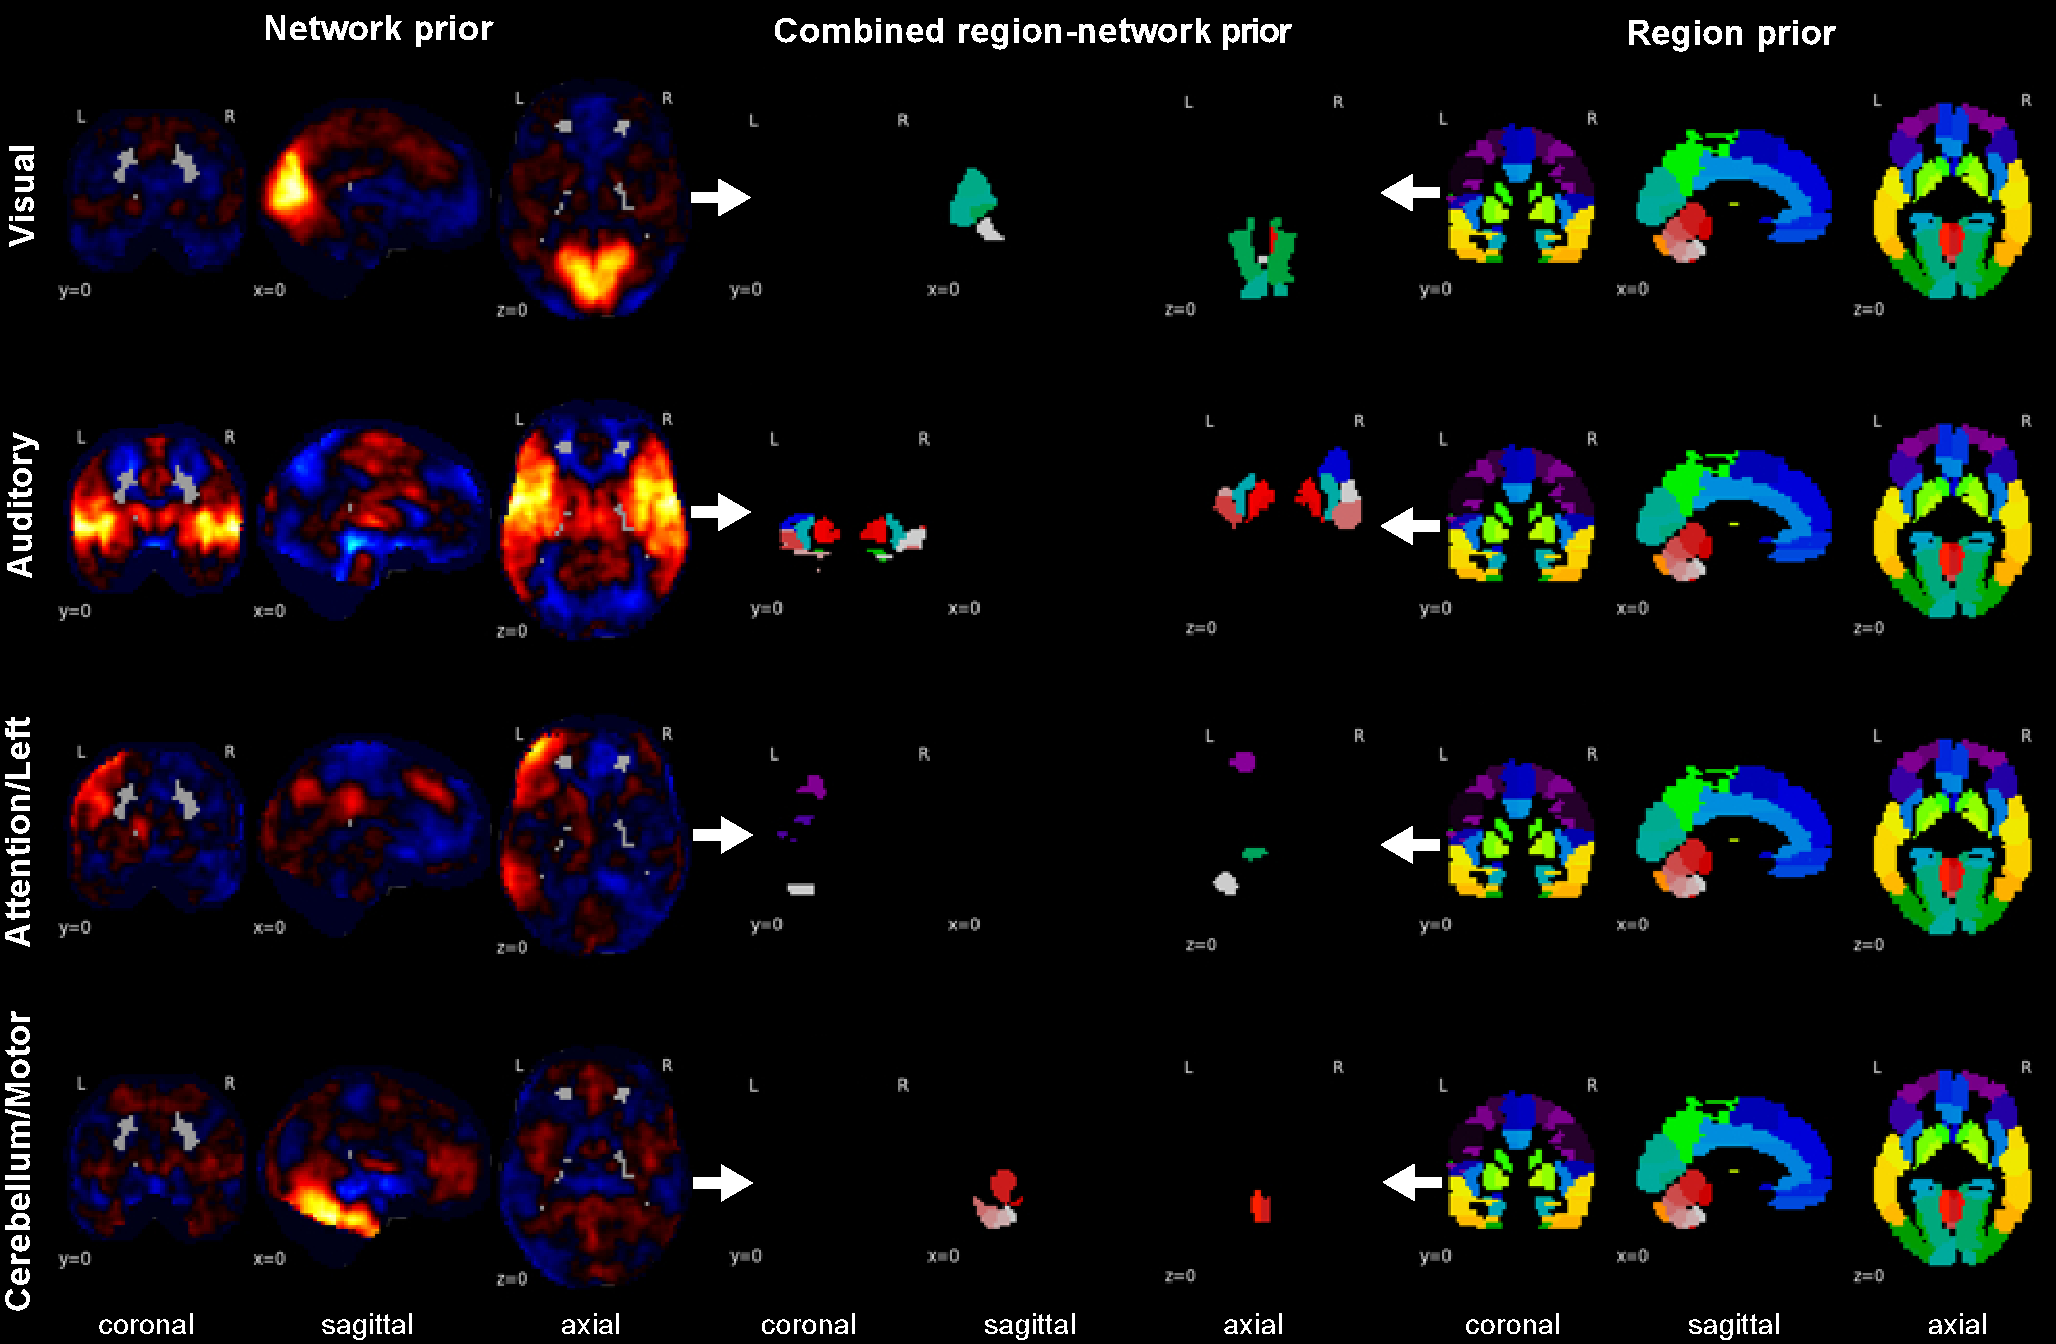
\includegraphics[width=1.00\textwidth]{figures/reg_net_prior.pdf}
\end{centering}
\vspace{-0.6cm}
\caption{\textbf{Building blocks of the region-network tree.}
Depicts neurobiological priors introduced into the supervised classification
by hierarchical structured sparsity.
\textit{Left:} Continuous, partially overlapping brain network priors
(\textit{hot-colored}, taken from \cite{smith2009})
accommodate the functional integration
perspective of brain organization.
\textit{Right:} Discrete, non-overlapping brain region priors
(\textit{single-colored}, taken from \cite{crad12})
accommodate the functional segregation perspective.
\textit{Middle:} These two types of predefined voxel groups are incorporated
into hierarchical priors of parent networks with their
descending region nodes.
\textit{Top to bottom:} Four examplary region-network priors
are shown, including
the early cortex that processes
visual and sound information from the environment,
a well-known attentional circuit in the left brain hemisphere,
and
the cerebellum that realizes motor behavior.
}
\label{fig_priors}
\end{figure}


\begin{figure}
\begin{centering}
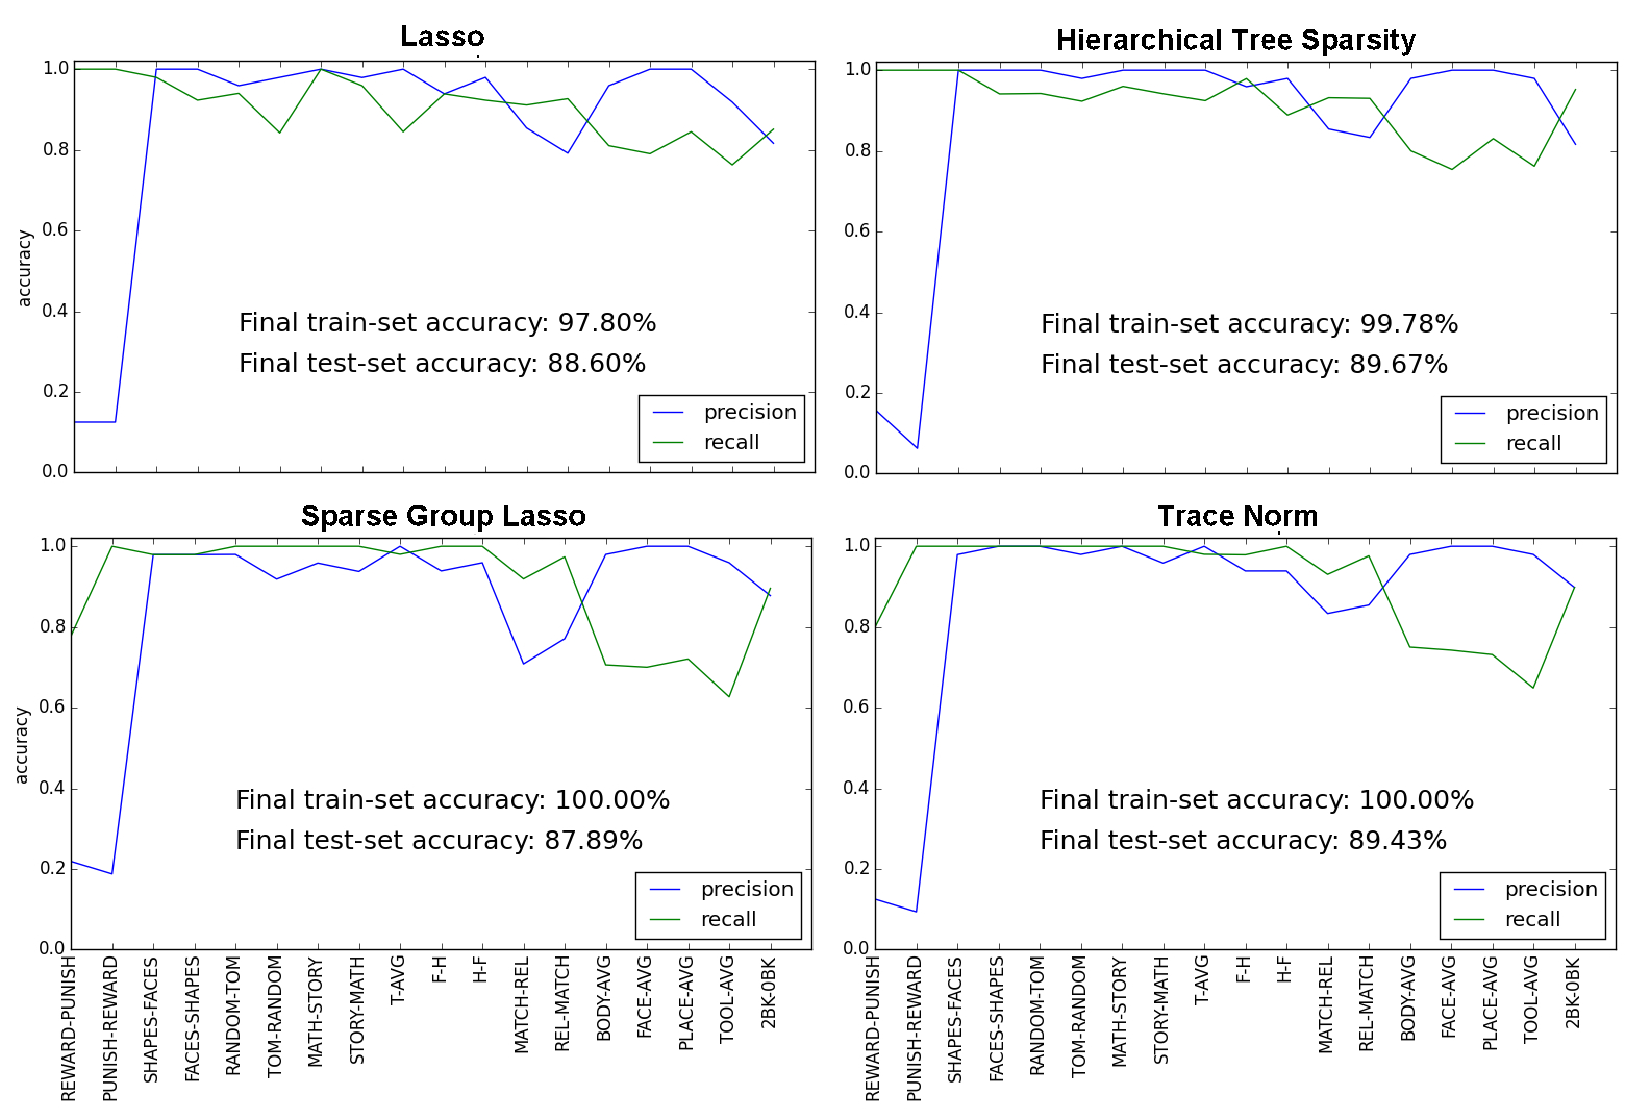
\includegraphics[width=1.00\textwidth]{figures/sparsities.pdf}
\end{centering}
\vspace{-0.6cm}
\caption{\textbf{Model performance across sparsity priors.}
Compares the performance of 4 logistic regression estimators
with different structured and unstructered sparsity terms
in classifying neural activity from 18 psychological tasks.
The class-wise precision and recall metrics
were obtained on the test set.
%
Unstructured $\ell_1$-penalized logistic regression (\textit{upper left})
imposed a minimum of relevant brain voxels without
assuming special structure.
Structured $\ell_1/\ell_2$ block norm with additional $\ell_1$ term
(\textit{lower left})
imposed region compartments, but na\"ive to network structure.
Structured trace-norm penalization (\textit{lower tight})
imposed low-rank structure
with sparsity of network patterns, but na\"ive to region structure.
Structured $\ell_1/\ell_2$ block norm with a hierarchy of
both region and network priors (\textit{upper tight})
exhibited the best out-of-sample performance.
%
Consequently, a priori knowledge of both region and network neighborhoods
was the most beneficial structured sparsity penalty.
}
\label{fig_sparsities}
\end{figure}


\paragraph{Benchmarking hierarchical tree sparsity against
common sparsity penalties.}
Hierarchical region-network priors have been systematically
evaluated against other popular choices of sparse classification algorithms
in an 18-class scenario
(Figure \ref{fig_sparsities}).
%
Logistic regression with $\ell_1/\ell_2$ block norm penalization
incorporated a hierarchy of previously known region and network neighborhoods
for a neurobiological bias of the statistical estimation.
%
Vanilla logistic regression with $\ell_1$-penalization
does not assume any previously known special structure.
This classification estimator embraces a vision of neural activity structure
that expectes a minimum of
topographically and functionally independent brain voxel to be relevant.
%
Logistic regression with sparse group sparsity
imposes a structured $\ell_1/\ell_2$ block norm with additional $\ell_1$ term
with a known atlas of region voxel groups onto the statistical estimation process.
This supervised estimator shrinks and selects the coefficients
of topographically compact voxel groups expected to be relevant together.
%
Logistic regression with trace-norm penalization
imposed low-rank structure.
This supervised classification algorithm
expected a minimum of unknown network patterns
to be relevant.
%
The stratified and shuffled training data were submitted to
to a nested cross-validation scheme
for model selection and model assessment.
In the inner CV layer, the logistic regression estimators
have been trained in a one-versus-rest design that
distinguishes each class from
the respective 17 other classes
(number of maximal iterations=$100$, tolerance=$0.001$).
In the outer CV layer, grid search
selected among candidates for the respective $\lambda$ parameter
by searching between $10^{-2}$ and $10^{1}$ in 9 steps on a logarithmic scale.
Importantly, the thus selected sparse logistic regression classifier was
evaluated on an identical test set in all settings.
%
Hierarchial tree sparsity demonstrated the best generalization
in distinguihsing unseen neural activity maps from 18 tasks
(89.67\%, mean recall XX.YY, mean precision XX.YY).
It was closely followed by logistic regression with trace-norm
regularization that is structured but not neurobiologically informed
(89.43\%, mean recall XX.YY, mean precision XX.YY).
Lasso featured an average performance comparing to the other sparse estimators
(88.60\%, mean recall XX.YY, mean precision XX.YY)
Introduced a priori knowledge of brain region compartments
by sparse group sparsity performed worst
(87.89\%, mean recall XX.YY, mean precision XX.YY).
%
In sum,
biasing sparse model selection by domain knowledge of region-network hierarchies
outperformed other types of frequently used sparse penalization techniques.



\begin{figure}
\begin{centering}
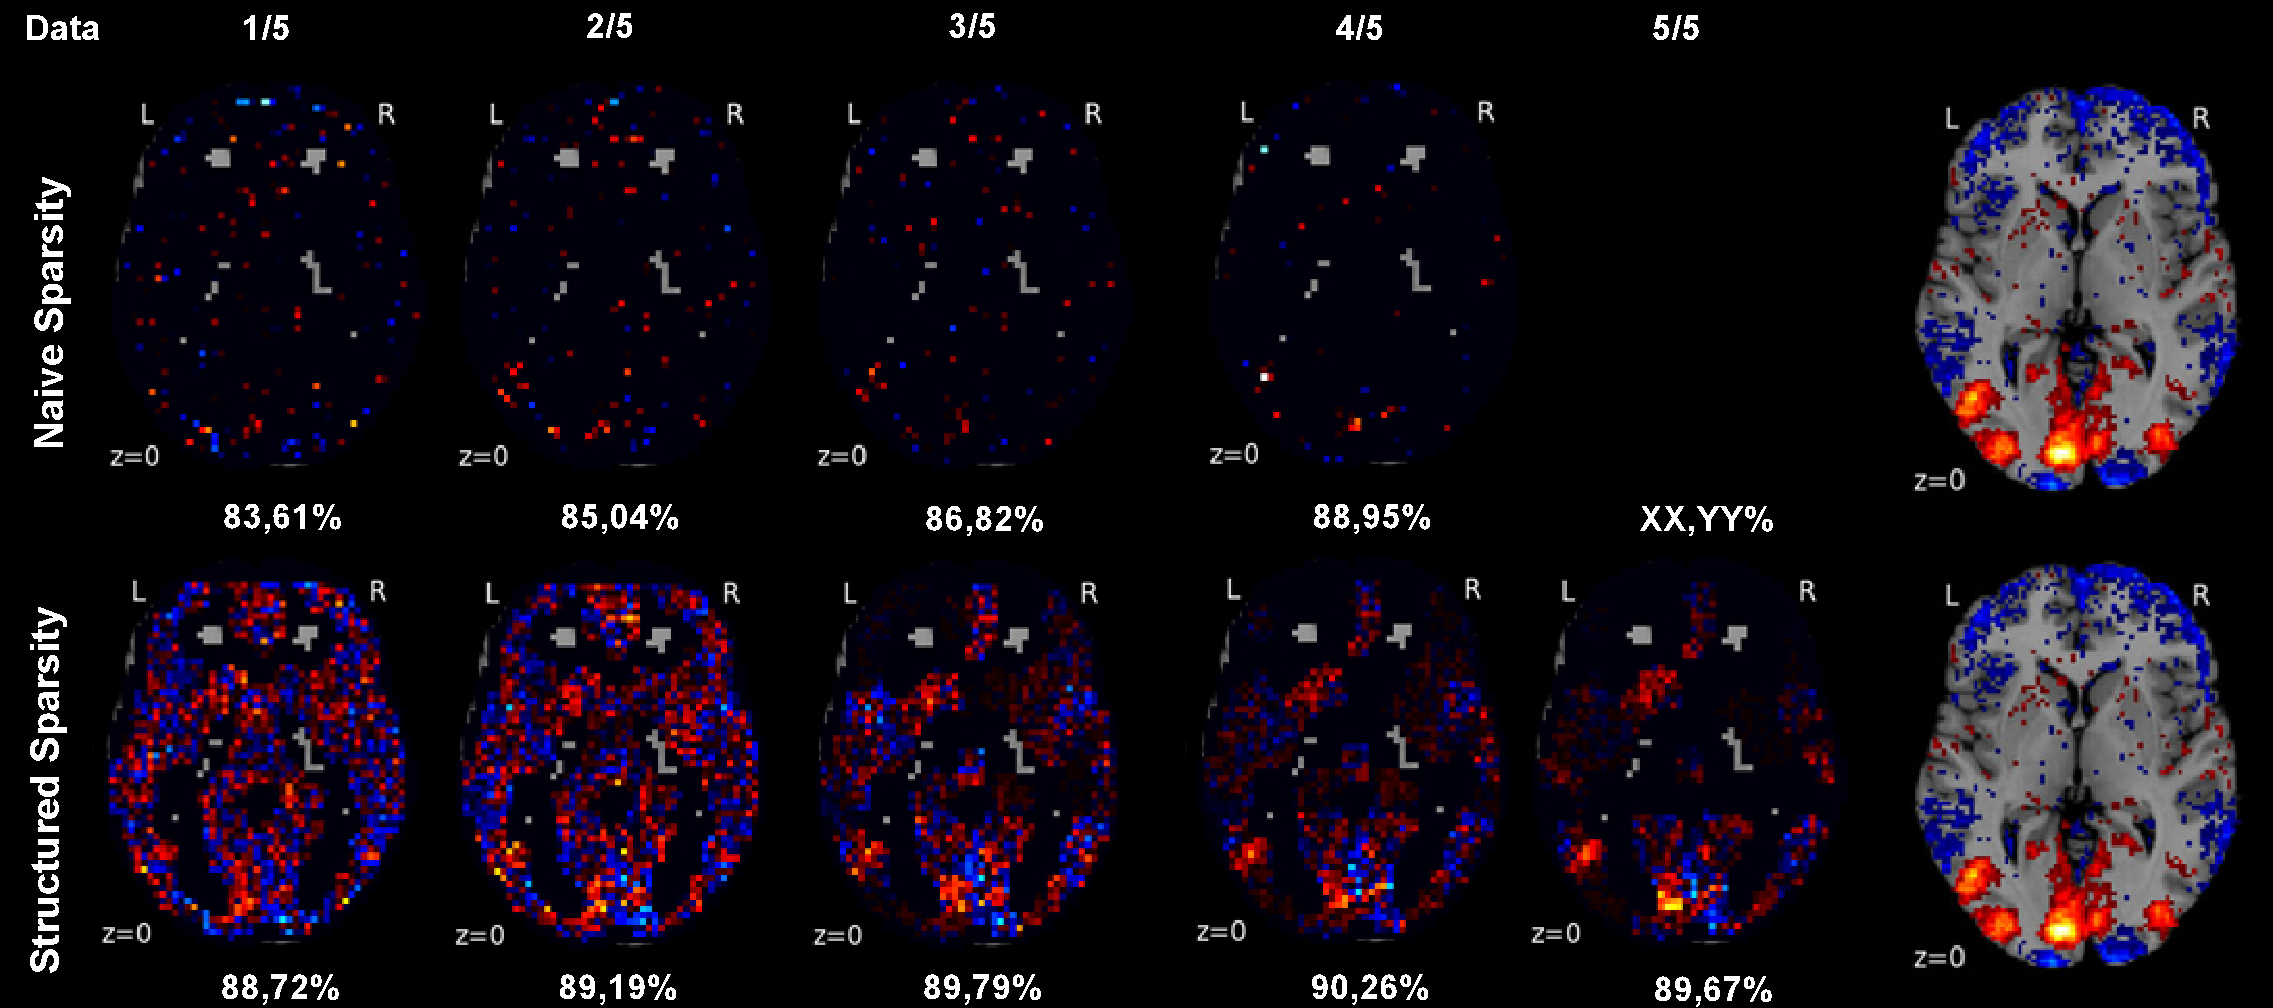
\includegraphics[width=1.00\textwidth]{figures/dataratio.pdf}
\end{centering}
\vspace{-0.6cm}
\caption{\textbf{Na\"ive versus informed sparse model selection
across training set sizes.}
Ordinary $\ell_1$-penalized logistic regression
(\textit{upper row})
is compared
to hierarchical-tree-penalized logistic regression
(\textit{lower row})
with increasing fraction
of the available training data (\textit{columns}).
For one example from 18 classes,
unthresholded axial maps of model weights
are shown for comparison against
the class sample average {\color{red} thresholded at p $<$ 0.01 ???}
in the \textit{rightmost column}.
The corresponding 18-class (``View tools'')
out-of-sample accuracy
is given in percent.
%
In the data-scarce scenario,
typical for brain imaging,
hierarchical tree sparsity achieves
better support recovery with the biggest difference
in model performance.
%
In the data-rich scenario,
neurobiologically informed logistic regression
profits more from the increased information quantities than
neurobiologically naive logistic regression.
}
\label{fig_dataratio}
\end{figure}



\paragraph{Sample complexity of na\"ive versus informed sparse model selection.}
Subsequently, the sample complexity of
$\ell_1$-penalized and hierarchical-tree-penalized logistic regression
were quantitatively compared (Figure \ref{fig_dataratio}).
Region-network priors should bias model selection towards more
neurobiologically plausible classification estimators.
This should yield better out-of-sample generalization and
support recovery than
$\ell_1$-constrained logistic regression na\"ive to neurobiology
in the data-scarce and data-rich scenarios.
%
The HCP task data with examples from 18 classes were first divided into
90\% of training set (i.e., 7584 neural activity maps) and
10\% of test set (i.e., 842 maps).
Both learning algorithms were fitted based on the
training set at different subsampling fractions:
20\% (1516 maps),
40\% (3033 maps),
60\% (4550 maps),
80\% (6067 maps), and
100\% (7584 maps).
%
The stratified and shuffled training data were submitted to
to a nested cross-validation scheme
for model selection and model assessment.
In the inner CV layer, the logistic regression estimators
have been trained in a one-versus-rest design that
distinguishes each class from
the respective 17 other classes
(number of maximal iterations=$100$, tolerance=$0.001$).
In the outer CV layer, grid search
selected among candidates for the respective $\lambda$ parameter
by searching between $10^{-2}$ and $10^{1}$ in 9 steps on a logarithmic scale.
Importantly, the thus selected sparse logistic regression classifier was
evaluated on an identical test set in all settings.
%
Three observation have been made.
In the data-scarce scenario (i.e., 1/5 of actual training data),
hierarchical tree sparsity achieved the biggest advantage
in out-of-sample performance by 5,11\% as well as
better support recovery with weight maps already much closer
to the training data average.
In the case of scarce training data, which is typical for the brain imaging domain,
regularization by region-network priors indeed allowed for
more effective extraction of classification-relevant structure
from the neural activity scans.
%
Across scenarios,
the weight maps from ordinary logistic regression exhibit
higher variance and many more zero coefficients
than hierarchical tree logistic regression.
Given the usually high multicollinearity in neuroimaging data,
this observation is likely to reflect instable selection of
representatives among class-responsive predictor groups
due to the $\ell_1$-norm penalization.
%
In the data-rich scenario (i.e., entire training data used for model fitting),
neurobiologically informed logistic regression
profits more from the increased information quantities than
neurobiologically naive logistic regression.
That is, the region-network priors actually further enhance the similarity
to the weight maps even in abundant input data.
This was the case although
the maximal classification performance of $\approx$90\% has already
been reached with small training data fractions by the structured estimator.
In contrast, 
the unstructured estimator reached this generalization performance
only with bigger input data quantities.


\begin{figure}
\begin{centering}
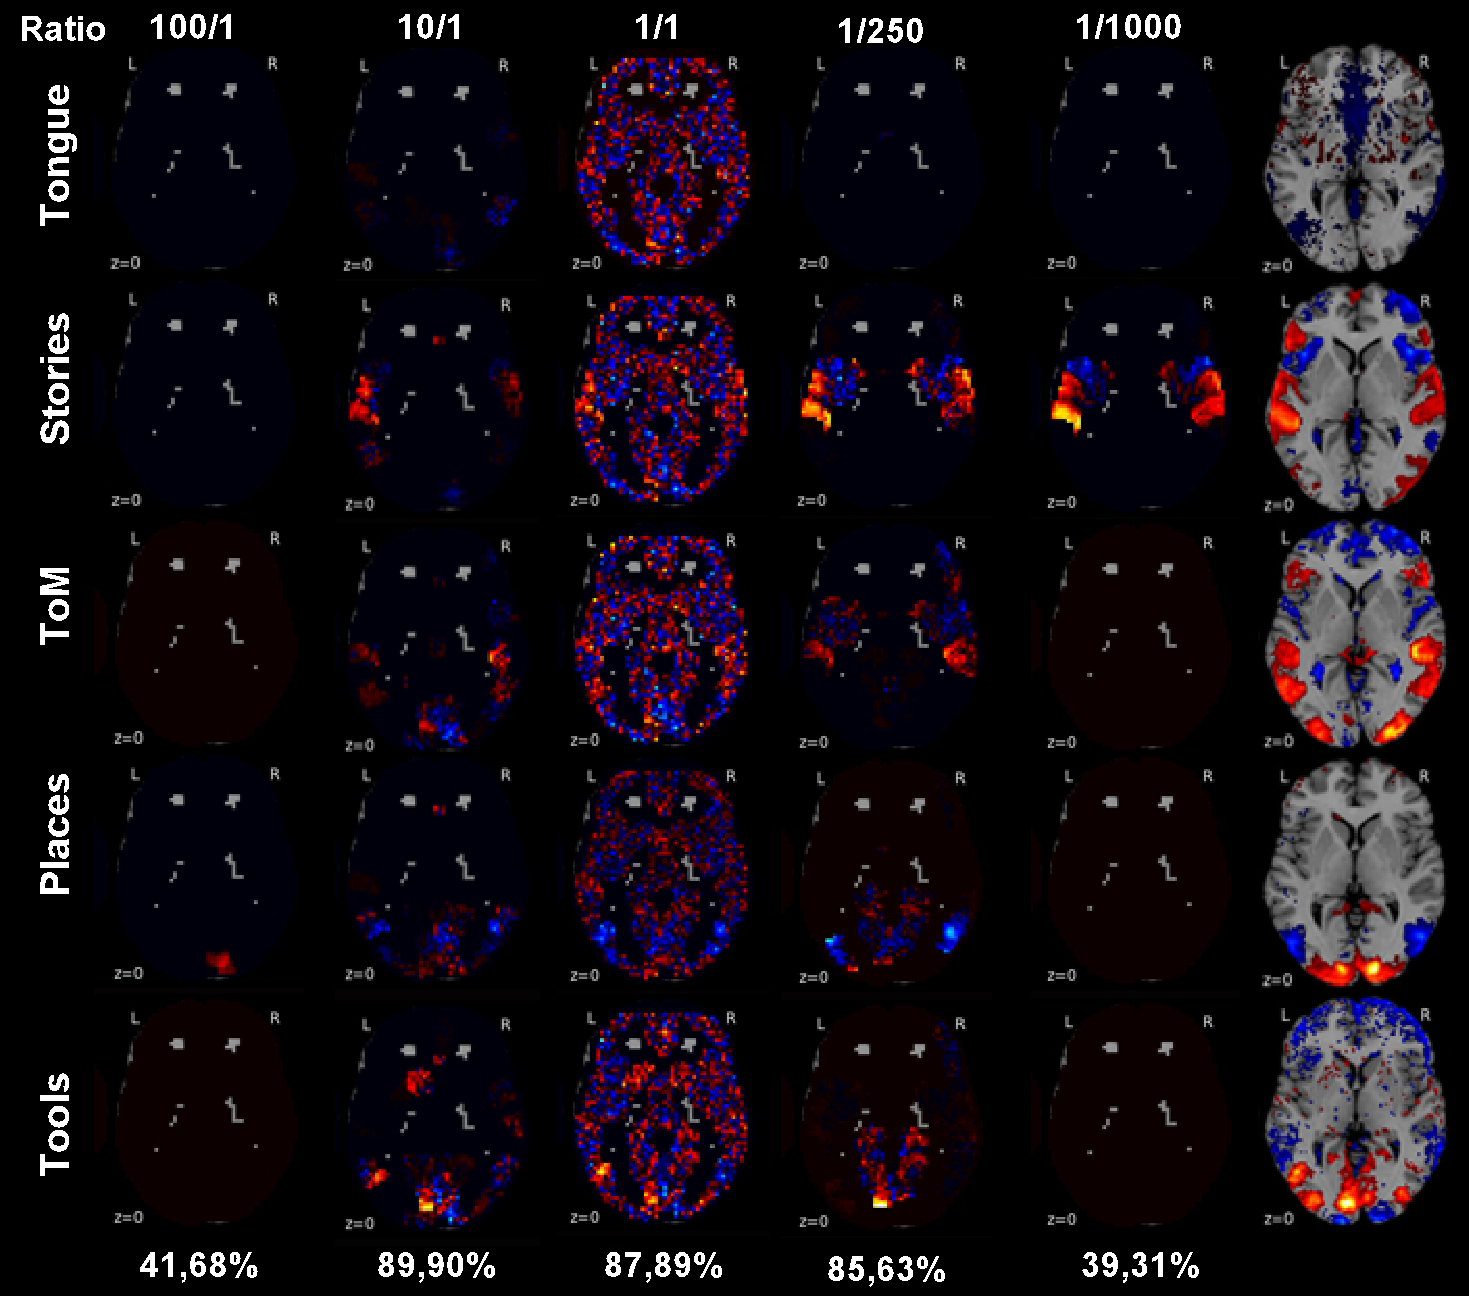
\includegraphics[width=1.00\textwidth]{figures/reg_net_ratio.pdf}
\end{centering}
\vspace{-0.6cm}
\caption{\textbf{Support recovery as a function of
region and network emphasis.}
The relative impact of the region and network priors
on model selection
is systematically varied against each other.
This region-network ratio (\textit{upper row}) weighted voxel groups
to priviledge sparse models in function space
that acknowledge known brain region neighborhoods
(\textit{left columns}) or
known brain networks compartments
(\textit{right columns}).
Among the 18 classes, the model weights are shown for the
tasks (\textit{from top to bottom}): tongue movement, listening stories,
taking somebody else's perspective (ToM, "theory of mind"),
as well as
viewing locations and tools.
The 18-class out-of-sample accuracy is indicated
on the \textit{bottom} and
the class-wise mean neural activty
in the \textit{rightmost column}.
%
Different emphasis on regions versus networks
in hierarchical structured sparsity can
yield essentially similar model performance.
%
Priviledging region versus network structure during model selection
recovers complementary aspects of the brain activity pattern.
%
Equal region and network emphasis yields more dispersed,
less interpretable predictive model choices.
}
\label{fig_regnetratio}
\end{figure}


\paragraph{Support recovery as a function of region and network emphasis.}
Finally, the relative importance of the
region and network priors within the hierarchical tree prior
was quantified (Figure \ref{fig_regnetratio}).
The $\eta_g$ group of region priors was multiplied with a
region-network ratio, while the
$\eta_g$ group of network priors was biased by the corresponding
network-region ratio. A region-network ratio of 3, for instance,
increased the relative importance of known region structure
by multiplying $\frac{3}{1}$ to the
$\eta_g$ factor of all region groups
and multiplying
$\frac{1}{3}$ to all network groups.
The data splitting cross-validation scheme was identical to the
above modelling experiments.
%
As the most important observation,
a range between region-dominant and network-dominant structured penalties
yields quantitatively almost identical generalization to new data
but qualitatively different decision functions manifested in the weight maps
(Figure \ref{fig_regnetratio}, second and forth column).
Classification models with many zero coefficients but high absolute
coefficients in either region compartments or network compartments
can similarly extrapolation to unseen neural activity maps.
Second,
these perform similar to equilibrated region-network priors
that set less voxel coefficients to zero and spread the
probability mass with lower absolute coefficients across the whole brain
(Figure \ref{fig_regnetratio}, third column in the middle).
Third,
overly strong emphasis on either level of the hierarchical prior
can yield the neurobiologically informative maps
of the most necessary region or network structure for
statistically significant out-of-sample performance
(Figure \ref{fig_regnetratio}, leftmost and rightmost columns).
%
In sum,
stratifying the hierarchical tree penalty between region and network emphasis
suggests that \textit{class-specific region-network weights}
might offer more performant and more interpretable classification models
in the future.



\section{Discussion}
Relevant structure in brain imaging data has long been investigated
separately
according to two distinct organizational principles:
functional segregation into discrete brain regions
and functional integration by interregional brain networks.
%
This paper demonstrates the simultaneous exploitation of
both these neurobiological compartments
for sparse variable selection and high-dimensional prediction
in a reference dataset.
%
Introducing existing domain knowledge into model selection
allowed privileging members of the function space
that are most neurobiologically plausible.
%
Domain-informed hierarchical structured sparsity is shown to enhance
both model interpretability and generalization performance,
although these statistical-learning goals are typically in conflict.



The present approach has important advantages over previous
neuroimaging studies that capitalized on dimensionality reduction to harness
the curse of dimensionality.
They often used preliminary region-wise pooling functions
or regression against network templates
for subsequent supervised learning on the aggregated feature space.
Such two-step approaches of feature engineering and inference
\textit{i)} can only account for either functional specialization or
functional integration of brain organization,
\textit{ii)} depend on the ground truth being a region or network effect,
and
\textit{iii)} cannot issue individual coefficients for every brain voxels.
%
Hierarchical region-network sparsity overcomes these shortcomings
by estimating individual voxel contributions
while benefitting from their functional segregation and integration
to restrict statistical complexity.
%
Viewed from the bias-variance tradeoff,
our modification to logistic regression estimators
entailed a large decrease in model variance but only a modest
increase in model bias.
Viewed from the Vapnik-Chervonenkis dimensions,
this entailed a healthy decrease in the complexity capactity of the prediction model
with a higher chance of generalizing to unobserved data.



In the future,
region-network sparsity priors could be incorporated into various
pattern-learning methods in systems neuroscience.
%
This includes supervised methods for whole-brain classification and regression
with one or several target variables.
The principled regularization scheme could even inform
unsupervised structure discovery methods,
such as principal component analysis
\cite{jenatton2009structured}
and
k-means clustering \cite{witten2010framework}.
%
Additionally,
model regularization by hierarchical structured sparsity could be extended
from the spatial domain of neural activity to
priors of coherent spatiotemporal activity structure
\cite{gramfort2011tracking}.
%
Ultimately,
successful high-dimensional inference is
an important prerequisite
for predicting diagnosis,
disease trajectories, and treatment responses
in personalized psychiatry and neurology.



\paragraph{Acknowledgment.}
{\small The research leading to these results has received funding from the
European Union Seventh Framework Programme (FP7/2007-2013)
under grant agreement no. 604102 (Human Brain Project).
Data were provided by the Human Connectome Project.
Further support was received from
the German National Academic Foundation (D.B.),
the German Research Foundation (BZ2/2-1 and BZ2/3-1 to D.B.),
and the MetaMRI associated team (B.T., G.V.).
}

  
\small
% \bibliographystyle{plainnat}
\bibliographystyle{splncs03}
\bibliography{paper_refs}



\end{document}
